\chapter{The LHCb detector}

The data used in this thesis originates from the LHCb detector, which is located at the LHC.
Therefore, this chapter first introduces the LHC and then describes the LHCb detector.

\section*{The LHC}

The LHC (Large Hadron Collider) is a $\qty{27}{\km}$ long ring accelerator located in the vicinity of Geneva at the border of France and Switzerland. 
It is the largest particle accelerator in the world, and it is managed by CERN (European Organization for Nuclear Research).
The LHC can collide protons with a center-of-mass energy of up to $\qty{14}{\TeV}$ at a peak luminosity (interactions per area and time) of $\qty{e34}{\cm\squared\s}$ \cite{LHC}.
Additionally, the LHC can also accelerate heavy ions.
The four largest detectors at the LHC are ATLAS, CMS, ALICE and LHCb.
While ATLAS and CMS are general-purpose particle detectors, ALICE is dedicated to heavy ion collisions resulting in a quark-gluon plasma.

\section*{The LHCb detector}

The LHCb detector is a particle detector dedicated to $pp$~collisions involving $c$ or $b$ quarks.
The goals of the LHCb collaboration are precision measurements of $C\!P$-violation and rare decays. 
To accomplish these goals, the LHCb detector has been build as a single arm forward-spectrometer covering angles to the beam pipe from $\qty{10}{\milli\radian}$ to $\qty{300}{\milli\radian}$ \cite{LHCb}. 
This design has been chosen because the majority of high energetic $b$-/$c$-hadron pairs, produced in $pp$~collisions, have Lorentz boosted velocities in the same direction as one of the incident protons.
An overview of the detector is shown in \autoref{fig:lhcb_detector}.
The following paragraphs briefly describe the components of the LHCb detector based on the article \cite{LHCb}.

\begin{figure}
    \centering
    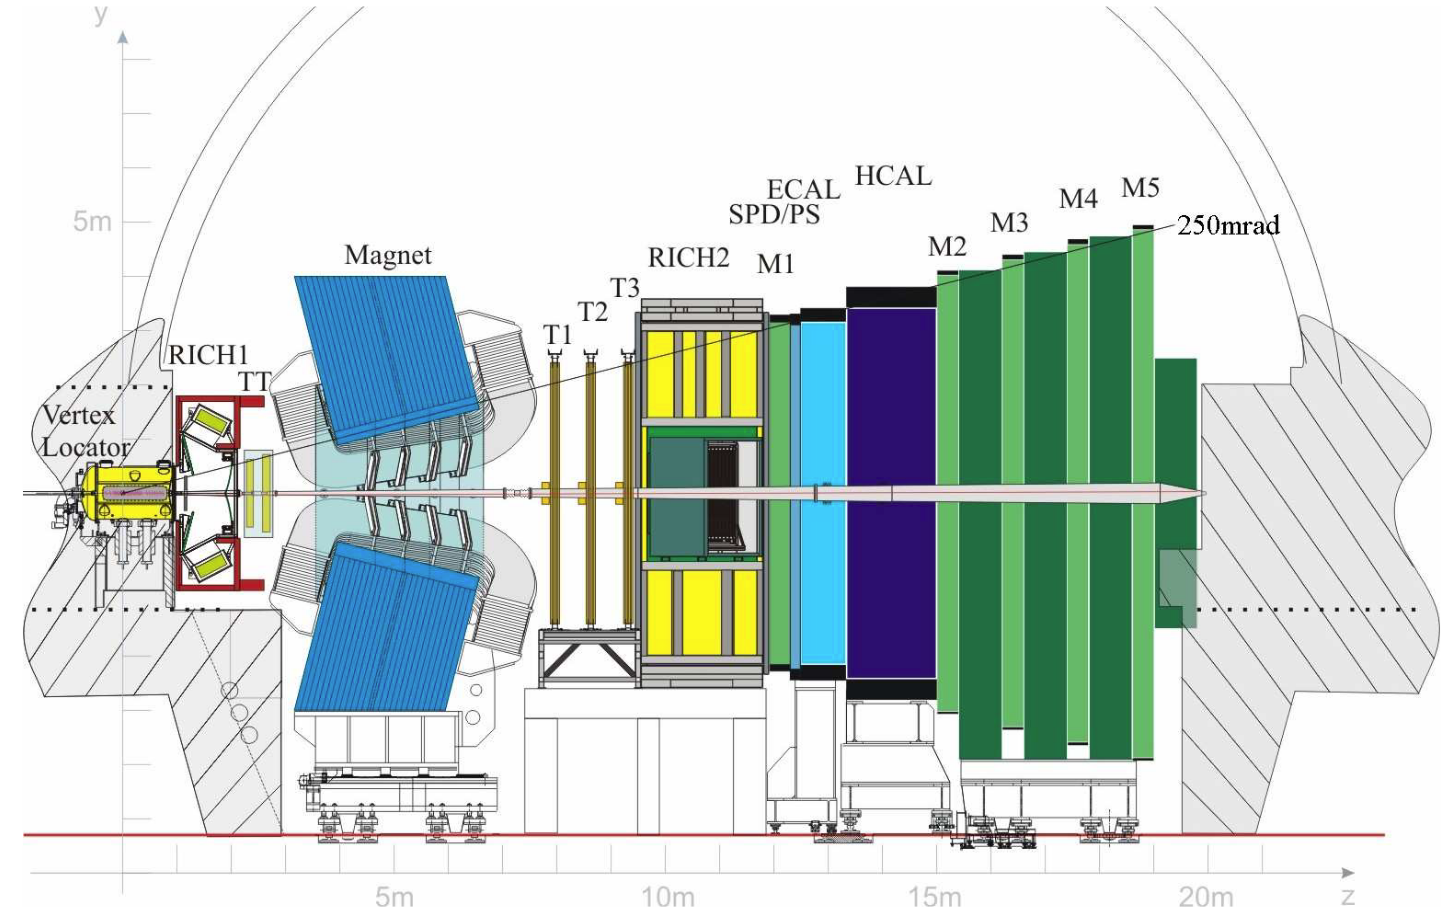
\includegraphics[width=\textwidth]{images/lhcb_detector.png}
    \caption{Sideview of the LHCb detector \cite{LHCb}. }
    \label{fig:lhcb_detector}
\end{figure}

A particle produced at the PV first traverses the Vertex Locator (VELO). 
There, the tracks of charged particles are measured using silicon semiconductor sensors at a resolution of about $\qty{4}{\micro\meter}$. 
This information then is primarily used to reconstruct the position of the primary and secondary vertices of the decay particles.

Beyond the VELO, the Tracking System then further measures the track points of the same particles. 
This is done in the Tracker Turicensis (TT) before the magnet and in the Trackers T1, T2 and T3 behind the magnet.
The dipole magnet bends the particle tracks through the Lorentz force so that the particle's momentum can be inferred.
While the TT and the inner parts of the T1-T3 also use silicon semiconductor sensors, the outer parts of the T1-T3 use straw-tube modules which are gaseous ionization detectors. 

The Ring Imaging Cherenkov detectors (RICH1, RICH2) are used to measure the particle velocities.
When charged particles traverse optically dense materials, the emission of Cherenkov radiation can be induced.
This radiation is then detected by photo multipliers. 
The opening angle of the emitted light cone is dependent on the velocity of the particle. 
The use of multiple radiators allows measuring particles with momenta between $\qty{1}{\GeV}$ and $\qty{100}{\GeV}$.
Comparing the momentum measured in the Tracking System with the velocity measured in the RICH detectors yields information particle's mass. 

The calorimeters (ECAL and HCAL) absorb and measure the energy of most particles.
In dense materials, particles can induce particle showers with the size directly related to the energy deposited.
Each calorimeter is structured in alternating layers of absorbers and scintillators. 
The electronic calorimeter~(ECAL) absorbs electrons, positrons and photons using lead, and the hadronic calorimeter~(HCAL) absorbs any hadrons using iron.
The pad/preshower detector~(SPD/PS) was used mostly in run 1 of the LHC to reject $\pi$~background detected in the ECAL.
The calorimeters are the only detectors at LHCb which can detect chargeless particles.

The muon chambers (M1-M5) track charged particles which pass through the calorimeters without absorption.
The majority of charged particles at this point in the detector are muons.
The iron layers between the muon chambers are used to absorb any non-muon particles.
M1-M5 are multi-wire proportional chambers to detect the track points of the muons.

The combined measured data of the RICH, the calorimeters and the muon chambers is used for particle identification.
Together with the Tracking System, this allows the reconstruction of the production and decay processes related to the $pp$-collision.

Due to the high precision of the LHCb detector, only a small portion of the $pp$-collisions visible in the LHCb detector can be permanently recorded for further analysis.
Therefore, a Trigger System is implemented to reduce the event detection rate from about $\qty{10}{\MHz}$ to about $\qty{2}{\kHz}$.
This system consists of the hardware trigger \enquote{Level-0}~(L0) and the software trigger \enquote{High Level Trigger}~(HLT).
The L0 collects information from the pile-up system of the VELO, the calorimeters and the muon chambers.
If the event does not contain particles with high transversal energy or momentum, it is rejected.
The L0 allows the readout of the whole detector at a rate of about $\qty{1}{\MHz}$.
The HLT then uses the data of all detector components to fully reconstruct the event and select events on various decision criteria.
At the final rate of about $\qty{2}{\kHz}$, the event data is permanently recorded and can then be accessed on demand by all members of the LHCb collaboration.
